\begin{frame}{Los intereses bajaron a 2,8\% del PIB en 2025}
\centering
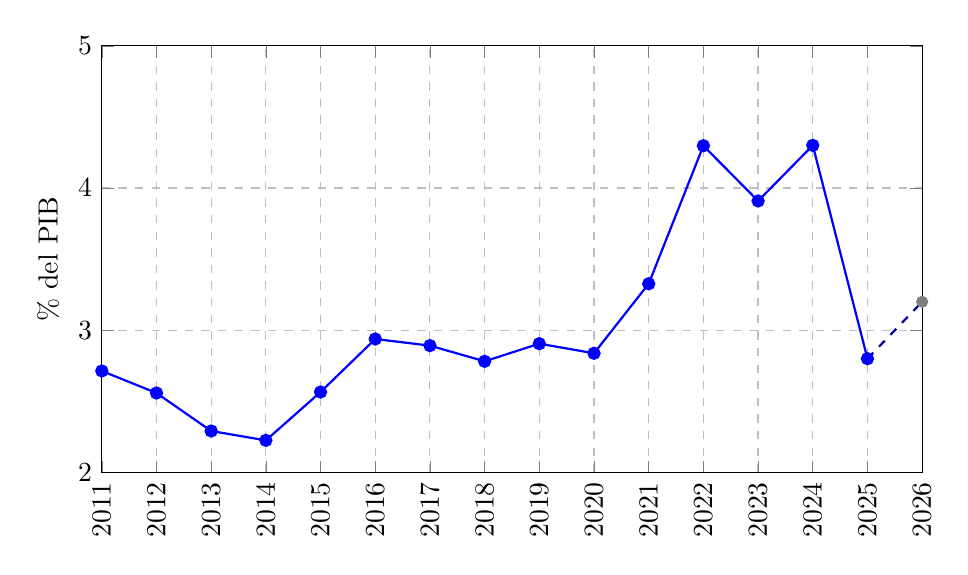
\begin{tikzpicture}
\begin{axis}[
    width=12cm,height=7cm,
    ylabel={\% del PIB},
    ymin=2,ymax=5,
    xmin=2011,xmax=2026,
    xtick={2011,...,2026},
    xticklabel style={rotate=90,anchor=east,/pgf/number format/.cd,1000 sep={},fixed},
    grid=both,
    grid style=dashed
]
\addplot[solid,thick,blue,mark=*] coordinates {
(2011,2.7137) (2012,2.5585) (2013,2.2915) (2014,2.2256) (2015,2.5657)
(2016,2.9384) (2017,2.8917) (2018,2.7814) (2019,2.9055) (2020,2.8380)
(2021,3.3269) (2022,4.2975) (2023,3.9090) (2024,4.3) (2025,2.8)
};
\addplot[color=blue!60!black,dashed,thick] coordinates {(2025,2.8) (2026,3.2)};
\addplot[color=gray,mark=*,only marks] coordinates {(2026,3.2)};
\end{axis}
\end{tikzpicture}
\scriptsize Línea discontinua final: proyección 2026.
\note{[Sources] MFMP 2026, capítulo 1, tablas 1.3 y 1.5. Serie histórica previa: MHCP, como en la versión fuente.}
\end{frame}